\documentclass{thesis_proposal}
%\documentclass[singlespace]{thesis_proposal}
%\documentclass[doublespace]{thesis_proposal}

% If you don't like the citation style you get with the above, try
% uncommenting one of the following lines and using that instead.
%    \documentclass[square]{thesis_proposal}    %% cite with [] instead of ()
%    \documentclass[super]{thesis_proposal}     %% cite with superscripts

\usepackage{appendix}

% If you do not like the bibliography style provided by this package,
% comment out the next line and replace it with something you
% prefer ... and be sure to make an equivalent change
% to the bibliographystyle command, near the end of this file.
% Many styles are available on the web, but if you (or your
% committee have very specific requirements), you may
% be in for a lot of work, tailoring a file.
\usepackage{thesis_proposal_bib} % file provided with this package
\begin{document}

\frontmatter                    % do not delete this line

%*** Uncomment one of the following lines to indicate the degree being sought
%\msc
\phd
%***

\title[(Insert short title here)]{(Insert proposal title here)}

\author[(Insert short name here)]{(Insert student name here)}

%% Edit the next two lines to alter the logo. Use {} for each, for no logo.
%\logofile{logo-eagle}
%\logoscale{0.8}
\logofile{}
\logoscale{}

\previousdegree{(Insert previous degrees here, e.g. BSc (year) (institution) (thesis title))}

\submitdate{(fill in date)}

\submitmip{(fill in months in program)} % months in program, at submit date

\acceptdate{(fill in date)}

%*** Comment out the next line, if no defense was held
\defenddate{(fill in date)}
%***

\supervisor{(insert name of supervisor)}

\cosupervisor{(insert name of cosupervisor)}

\supervisorycommittee{(Insert names of supervisory committee members here, in alphabetical order.)}

%*** Comment out the next line, if no defense was held
\defensecommittee{(Insert names of examination committee members here, in alphabetical order.)}
%***

\defensechair{(Insert defense chair's name here)}

\maketitle

%% Insert keywords, and the the abstract.  Keep the abstract under
%% about 350 words, or the material on the first page may flow onto
%% the second page.  Note that there there is a word limit on theses,
%% so learning to write to a limit is not a bad thing!  Besides, your
%% committee will be more impressed by brevity than wordiness.

\begin{abstract}{keyword1; keyword2; keyword3; keyword4; keyword5}
Lorem ipsum dolor sit amet, consectetur adipisicing elit, sed do
eiusmod tempor incididunt ut labore et dolore magna aliqua. Ut enim ad
minim veniam, quis nostrud exercitation ullamco laboris nisi ut
aliquip ex ea commodo consequat.  Duis aute irure dolor in
reprehenderit in voluptate velit esse cillum dolore eu fugiat nulla
pariatur.  Excepteur sint occaecat cupidatat non proident, sunt in
culpa qui officia deserunt mollit anim id est laborum.
\end{abstract}

\mainmatter                     % do not delete this line

%% Possibly you'd like to uncomment some of the following blocks.
%
%\singlespacing\listoffigures
%\singlespacing\listoftables

\section{Lorem ipsum}

\subsection{In reprehenderit}

\begin{figure}[t]
  \begin{center}
    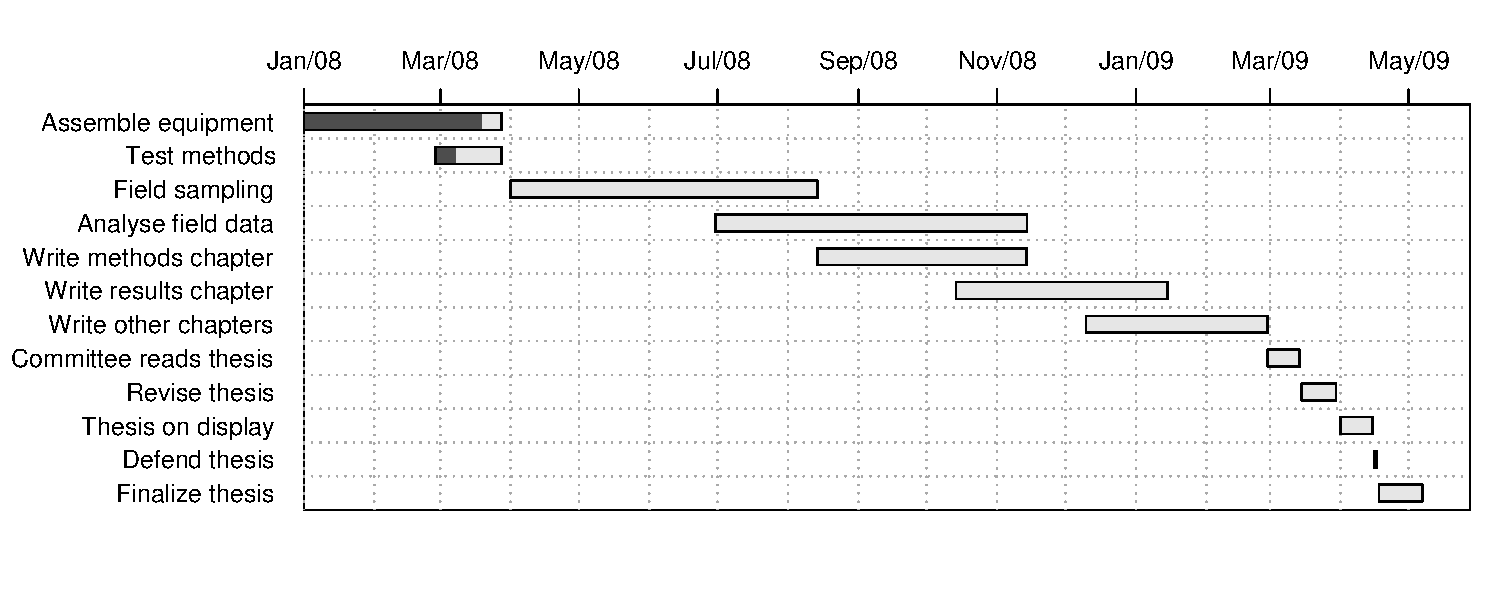
\includegraphics[width=\hsize]{planning} % using a default suffix
  \end{center}
  \caption[Research timetable.]{\label{f:planning}Thesis timetable, created
  with the data in Table~\ref{t:planningdata} using the R code in Table~\ref{t:planningR}. Oh, and here's some more text to make the caption longer, so we can test whether double spacing works ...}
\end{figure}

Referencing demonstrations:
equation \eqref{e:expansion};
Figure~\ref{f:planning};
Table~\ref{t:planningdata}.

Literature citation demonstrations:
article \cite{Voss:2001} \dots \cite[]{Voss:2001};
book \cite{JeffreysJeffreys1972}  \dots \cite[]{JeffreysJeffreys1972};
incollection \cite{Marshall1985}  \dots\cite[]{Marshall1985};
phdthesis \cite{Michel:1974} \dots \cite[]{Michel:1974}.

Multiple literature citation style:
\cite{Voss:2001,Jahnke:1990} \dots
\cite[]{Voss:2001,Jahnke:1990}.

Lorem ipsum dolor sit amet, consectetur adipisicing elit, sed do
eiusmod tempor incididunt ut labore et dolore magna aliqua. Ut enim ad
minim veniam, quis nostrud exercitation ullamco laboris nisi ut
aliquip ex ea commodo consequat. Duis aute irure dolor in
reprehenderit in voluptate velit esse cillum dolore eu fugiat nulla
pariatur. Excepteur sint occaecat cupidatat non proident

\begin{equation}
  \label{e:expansion}
  \alpha = -\frac{1}{\rho}\frac{\partial \rho}{\partial T},
\end{equation}

sunt in culpa qui officia deserunt mollit anim id est laborum. Lorem
ipsum dolor sit amet, consectetur adipisicing elit, sed do eiusmod
tempor incididunt ut labore et dolore magna aliqua. Ut enim ad minim
veniam, quis nostrud exercitation ullamco laboris nisi ut aliquip ex
ea commodo consequat. Duis aute irure dolor in reprehenderit in
voluptate velit esse cillum dolore eu fugiat nulla pariatur. Excepteur
sint occaecat cupidatat non proident, sunt in culpa qui officia
deserunt mollit anim id est laborum.  Lorem ipsum dolor sit amet,
consectetur adipisicing elit, sed do eiusmod tempor incididunt ut
labore et dolore magna aliqua. Ut enim ad minim veniam, quis nostrud
exercitation ullamco laboris nisi ut aliquip ex ea commodo
consequat. Duis aute irure dolor in reprehenderit in voluptate velit
esse cillum dolore eu fugiat nulla pariatur. Excepteur sint occaecat
cupidatat non proident, sunt in culpa qui officia deserunt mollit anim
id est laborum


Lorem ipsum dolor sit amet, consectetur adipisicing elit, sed do
eiusmod tempor incididunt ut labore et dolore magna aliqua. Ut enim ad
minim veniam, quis nostrud exercitation ullamco laboris nisi ut
aliquip ex ea commodo consequat. Duis aute irure dolor in
reprehenderit in voluptate velit esse cillum dolore eu fugiat nulla
pariatur. Excepteur sint occaecat cupidatat non proident, sunt in
culpa qui officia deserunt mollit anim id est laborum.

Lorem ipsum dolor sit amet, consectetur adipisicing elit, sed do
eiusmod tempor incididunt ut labore et dolore magna aliqua. Ut enim ad
minim veniam, quis nostrud exercitation ullamco laboris nisi ut
aliquip ex ea commodo consequat. Duis aute irure dolor in
reprehenderit in voluptate velit esse cillum dolore eu fugiat nulla
pariatur. Excepteur sint occaecat cupidatat non proident, sunt in
culpa qui officia deserunt mollit anim id est laborum. Lorem ipsum
dolor sit amet, consectetur adipisicing elit, sed do eiusmod tempor
incididunt ut labore et dolore magna aliqua. Ut enim ad minim veniam,
quis nostrud exercitation ullamco laboris nisi ut aliquip ex ea
commodo consequat.  Duis aute irure dolor in reprehenderit in
voluptate velit esse cillum dolore eu fugiat nulla pariatur. Excepteur
sint occaecat cupidatat non proident, sunt in culpa qui officia
deserunt mollit anim id est laborum.


\begin{table}[tp]
    \caption{\label{t:planningR}Source code to create
      Figure~\ref{f:planning}, based on the data in
      Table~\ref{t:planningdata}.  This uses the R package
      named \texttt{plan}, which is available on CRAN.}
  \begin{verbatim}
library(projectplanning)
library(projectplanning)
plan <- read.gantt("plan.dat")
pdf("planning.pdf", width=10, height=4)
plot(gantt)
  \end{verbatim}
\end{table}


\begin{table}[tp]
    \caption{\label{t:planningdata}Input data to create
      Figure~\ref{f:planning}, using the R code provided
      in Table~\ref{t:planningR}.
}
  \begin{verbatim}
"Assemble equipment"     2008-01-01 2008-03-28 90
"Test methods"           2008-02-28 2008-03-28 30
"Field sampling"         2008-04-01 2008-08-14  0
"Analyse field data"     2008-06-30 2008-11-14  0
"Write methods chapter"  2008-08-14 2008-11-14  0
"Write results chapter"  2008-10-14 2009-01-15  0
"Write other chapters"   2008-12-10 2009-02-28  0
"Committee reads thesis" 2009-02-28 2009-03-14  0
"Revise thesis"          2009-03-15 2009-03-30  0
"Thesis on display"      2009-04-01 2009-04-15  0
"Defend thesis           2009-04-16 2009-04-17  0
"Finalize thesis"        2009-04-18 2009-05-07  0
  \end{verbatim}
\end{table}


\subsection{Dolor sit amet}

Lorem ipsum dolor sit amet, consectetur adipisicing elit, sed do
eiusmod tempor incididunt ut labore et dolore magna aliqua. Ut enim ad
minim veniam, quis nostrud exercitation ullamco laboris nisi ut
aliquip ex ea commodo consequat. Duis aute irure dolor in
reprehenderit in voluptate velit esse cillum dolore eu fugiat nulla
pariatur. Excepteur sint occaecat cupidatat non proident, sunt in
culpa qui officia deserunt mollit anim id est laborum.

\subsubsection{Consectetur adipisicing}

Lorem ipsum dolor sit amet, consectetur adipisicing elit, sed do
eiusmod tempor incididunt ut labore et dolore magna aliqua. Ut enim ad
minim veniam, quis nostrud exercitation ullamco laboris nisi ut
aliquip ex ea commodo consequat. Duis aute irure dolor in
reprehenderit in voluptate velit esse cillum dolore eu fugiat nulla
pariatur. Excepteur sint occaecat cupidatat non proident, sunt in
culpa qui officia deserunt mollit anim id est laborum.

\subsubsection{Sed do eiusmod}

Lorem ipsum dolor sit amet, consectetur adipisicing elit, sed do
eiusmod tempor incididunt ut labore et dolore magna aliqua. Ut enim ad
minim veniam, quis nostrud exercitation ullamco laboris nisi ut
aliquip ex ea commodo consequat. Duis aute irure dolor in
reprehenderit in voluptate velit esse cillum dolore eu fugiat nulla
pariatur. Excepteur sint occaecat cupidatat non proident, sunt in
culpa qui officia deserunt mollit anim id est laborum.



\backmatter                     % do not delete this line
\appendix
\section{Tempor incididunt ut labore}

Lorem ipsum dolor sit amet, consectetur adipisicing elit, sed do
eiusmod tempor incididunt ut labore et dolore magna aliqua. Ut enim ad
minim veniam, quis nostrud exercitation ullamco laboris nisi ut
aliquip ex ea commodo consequat. Duis aute irure dolor in
reprehenderit in voluptate velit esse cillum dolore eu fugiat nulla
pariatur. Excepteur sint occaecat cupidatat non proident, sunt in
culpa qui officia deserunt mollit anim id est laborum.


\bibliographystyle{thesis_proposal}

\bibliography{literature} % uses file literature.bib in this directory

\end{document}
